\section{Results}

\subsection{Primary model comparison}
The regenerated temperature--salinity overview (Figure~\ref{fig:data_overview}) contains nonzero observations in all four named basins. The rank-1 model improved on the linear model in all four basins (Table~\ref{tab:model_performance}). Its temporal-validation RMSE was 20.172, 14.483, 16.002, and 10.575~$\umol$ in the Atlantic, Indian, Pacific, and Southern Ocean, respectively. The rank-2 minus rank-1 changes were +1.984, +0.254, $-0.289$, and $-0.035~\umol$ in the same order. Thus, adding four fitted parameters did not yield a consistent predictive improvement: rank-2 was worse in the Atlantic and Indian, and its improvements in the Pacific and Southern Ocean were small.

The full quadratic was less accurate than rank-1 in the Atlantic but improved slightly in the other three basins (Table~\ref{tab:model_performance}). Cubic models reduced validation RMSE further in the latter three basins, particularly the Indian, but used four times as many fitted coefficients. Figure~\ref{fig:model_hierarchy} shows the accuracy--complexity hierarchy.

\begin{figure}[htbp]
\centering
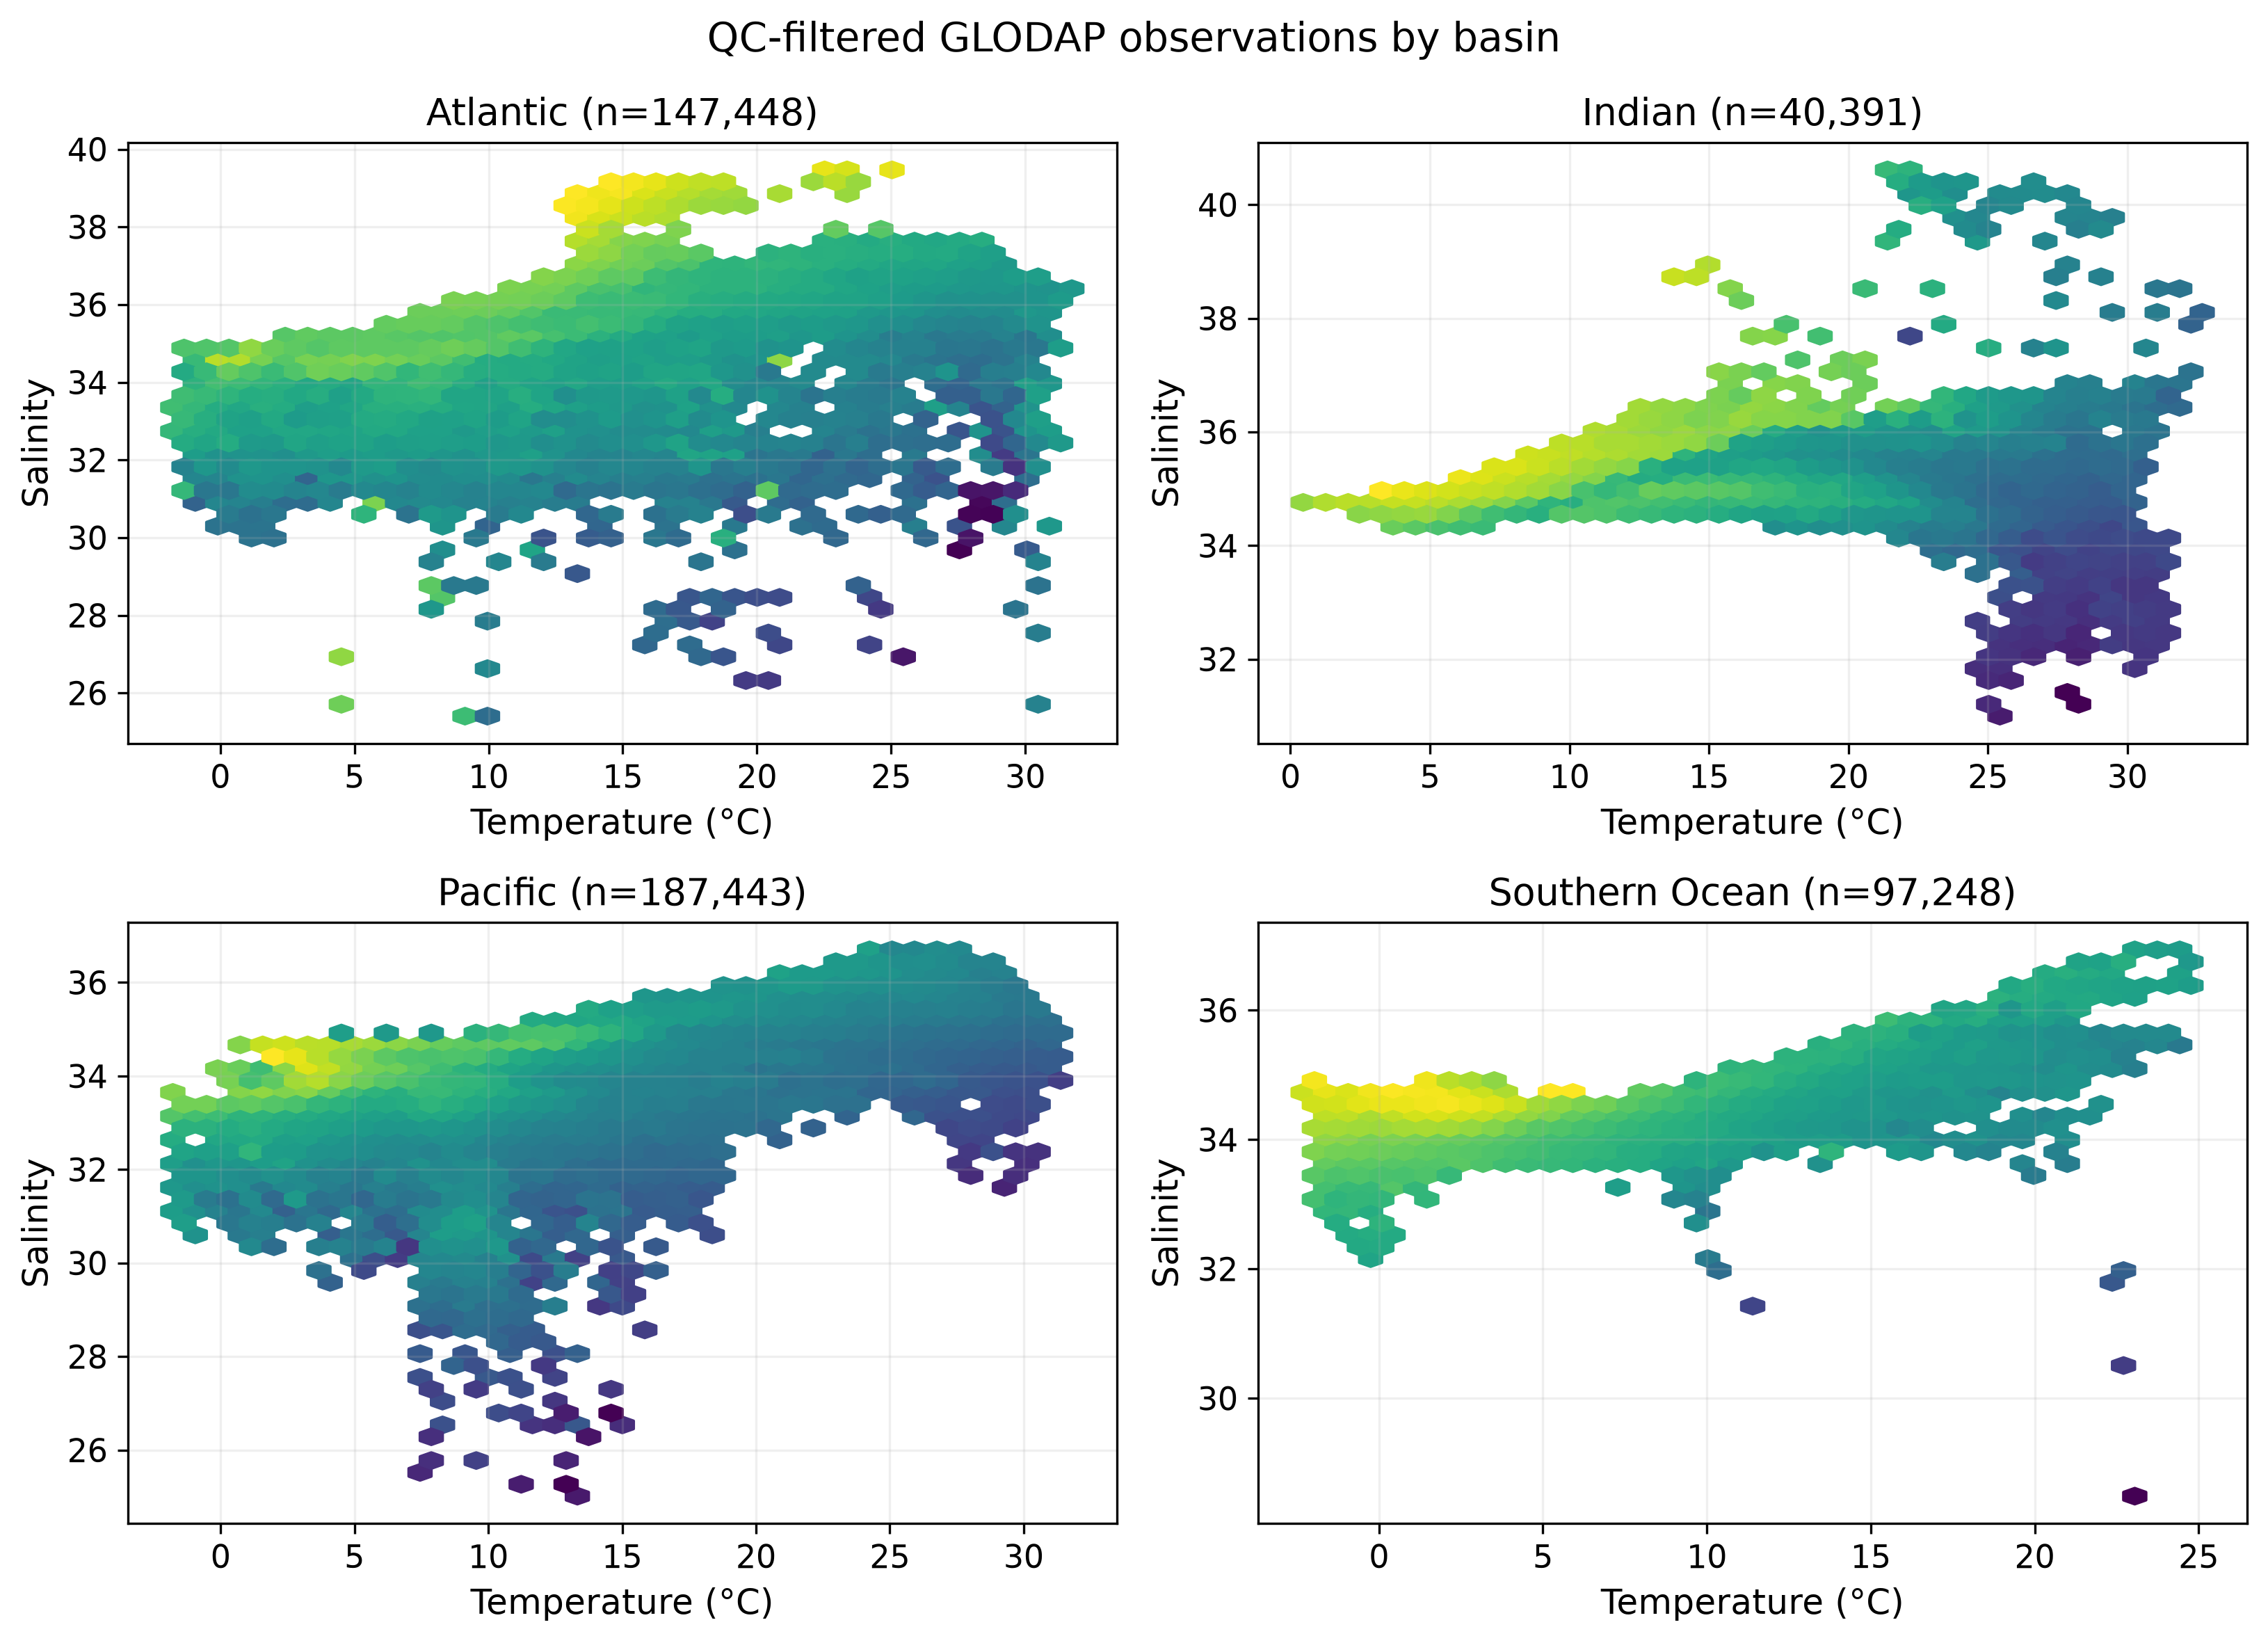
\includegraphics[width=\textwidth]{figures/figure1_data_overview.png}
\caption{Quality-controlled GLODAP observations in temperature--salinity space, colored by measured $\tco$. Panel counts are the four named-basin totals used in the analysis.}
\label{fig:data_overview}
\end{figure}

\begin{figure}[htbp]
\centering
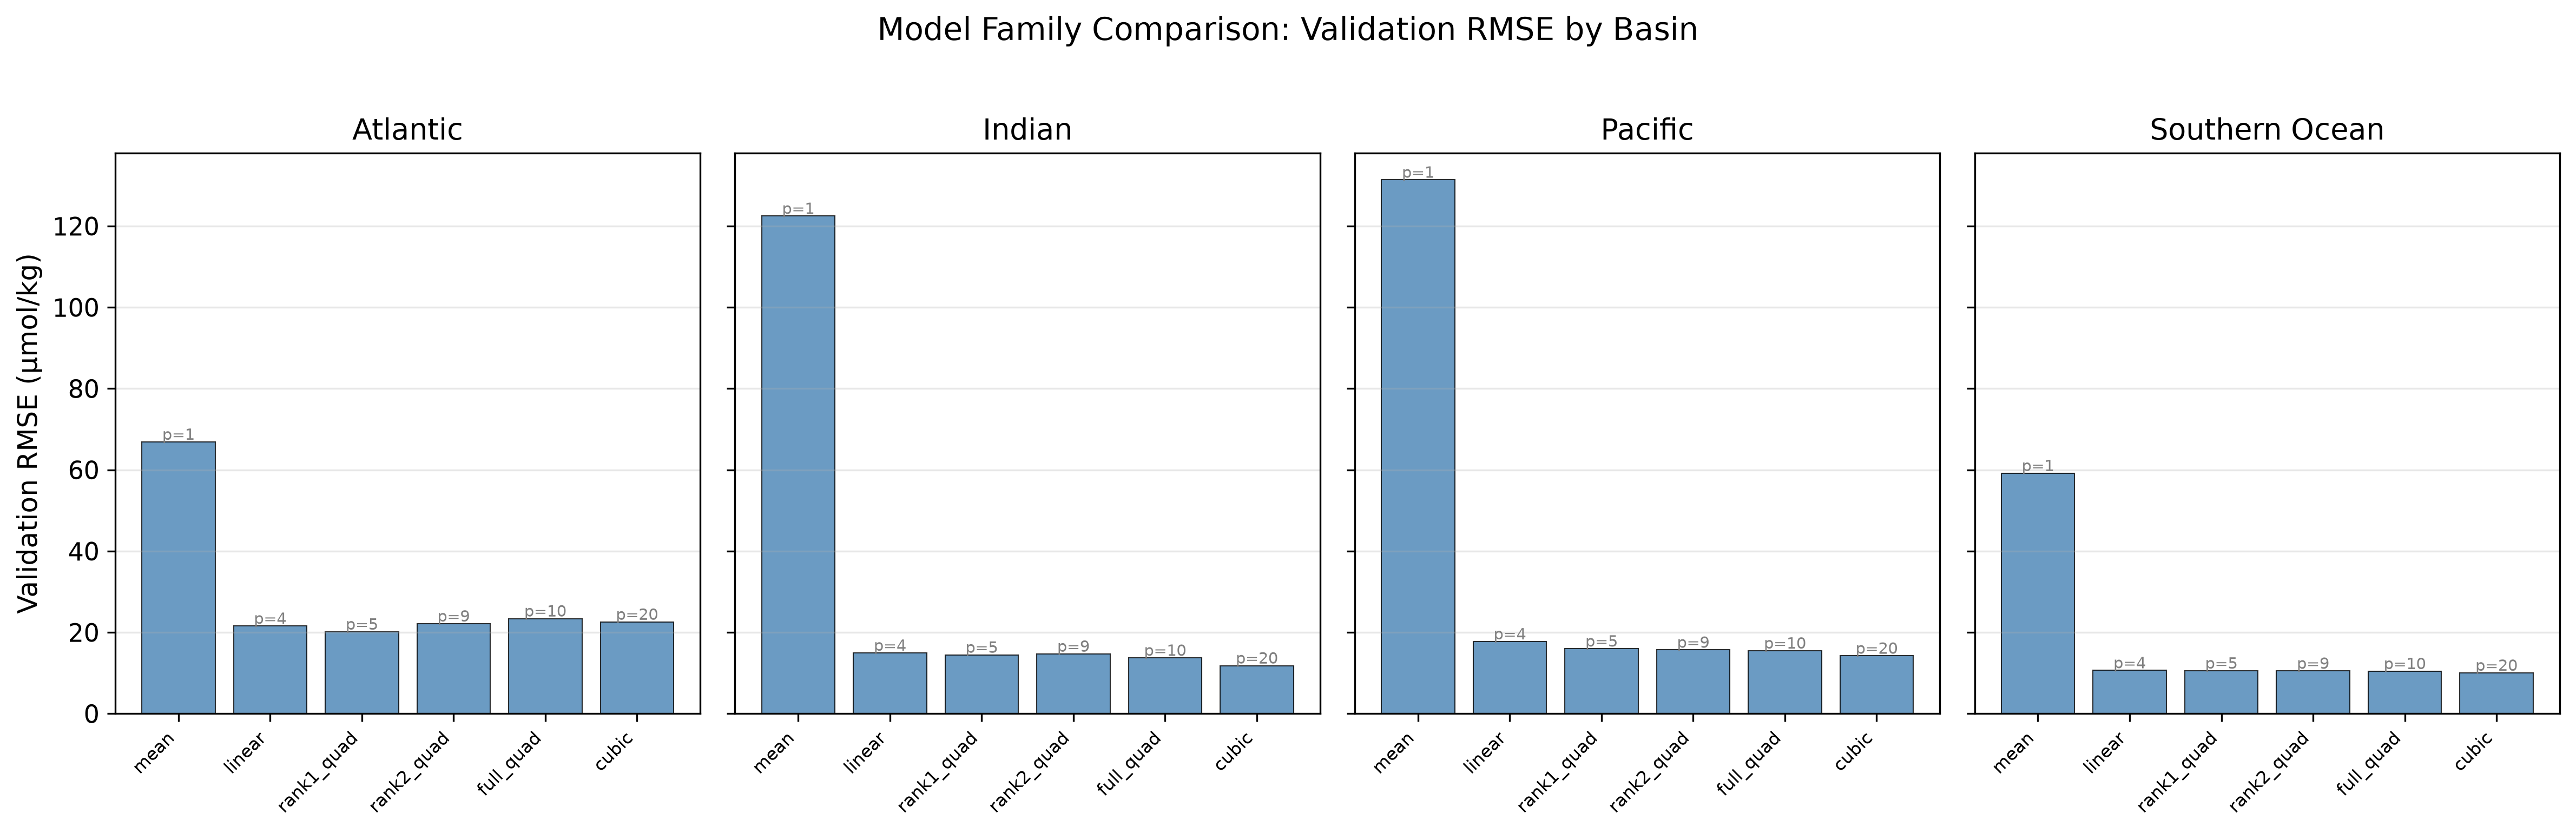
\includegraphics[width=\textwidth]{figures/figure2_model_hierarchy.png}
\caption{Temporal-validation RMSE for the predefined model families. Parameter counts are annotated in the source figure. The rank-1 model improves on the linear model in all basins but is not uniformly the most accurate family.}
\label{fig:model_hierarchy}
\end{figure}

\subsection{Symbolic recurrence and accuracy--complexity trade-off}
Rank-1 candidates occurred in 24 of 48 basin--operator--seed cells and in all four basins. Recovery was not operator-invariant: in the Atlantic, rank-1 candidates appeared only in the search space containing an explicit square operator. The count of 86 rank-1-classified rows includes repeated and syntactically classified candidates, so it should not be interpreted as 86 independent discoveries.

The best symbolic candidates improved validation RMSE relative to rank-1 by approximately 5.8\% in the Atlantic, 11.6\% in the Indian, 3.2\% in the Pacific, and 5.6\% in the Southern Ocean. Their complexities were 15, 25, 20, and 21, compared with $C=8$ for rank-1. Figure~\ref{fig:pareto} shows the trade-off: the compact model occupies the low-complexity end, while more complex expressions can improve accuracy. Rank-1 is therefore an efficient approximation rather than a universally preferred model.

\begin{figure}[htbp]
\centering
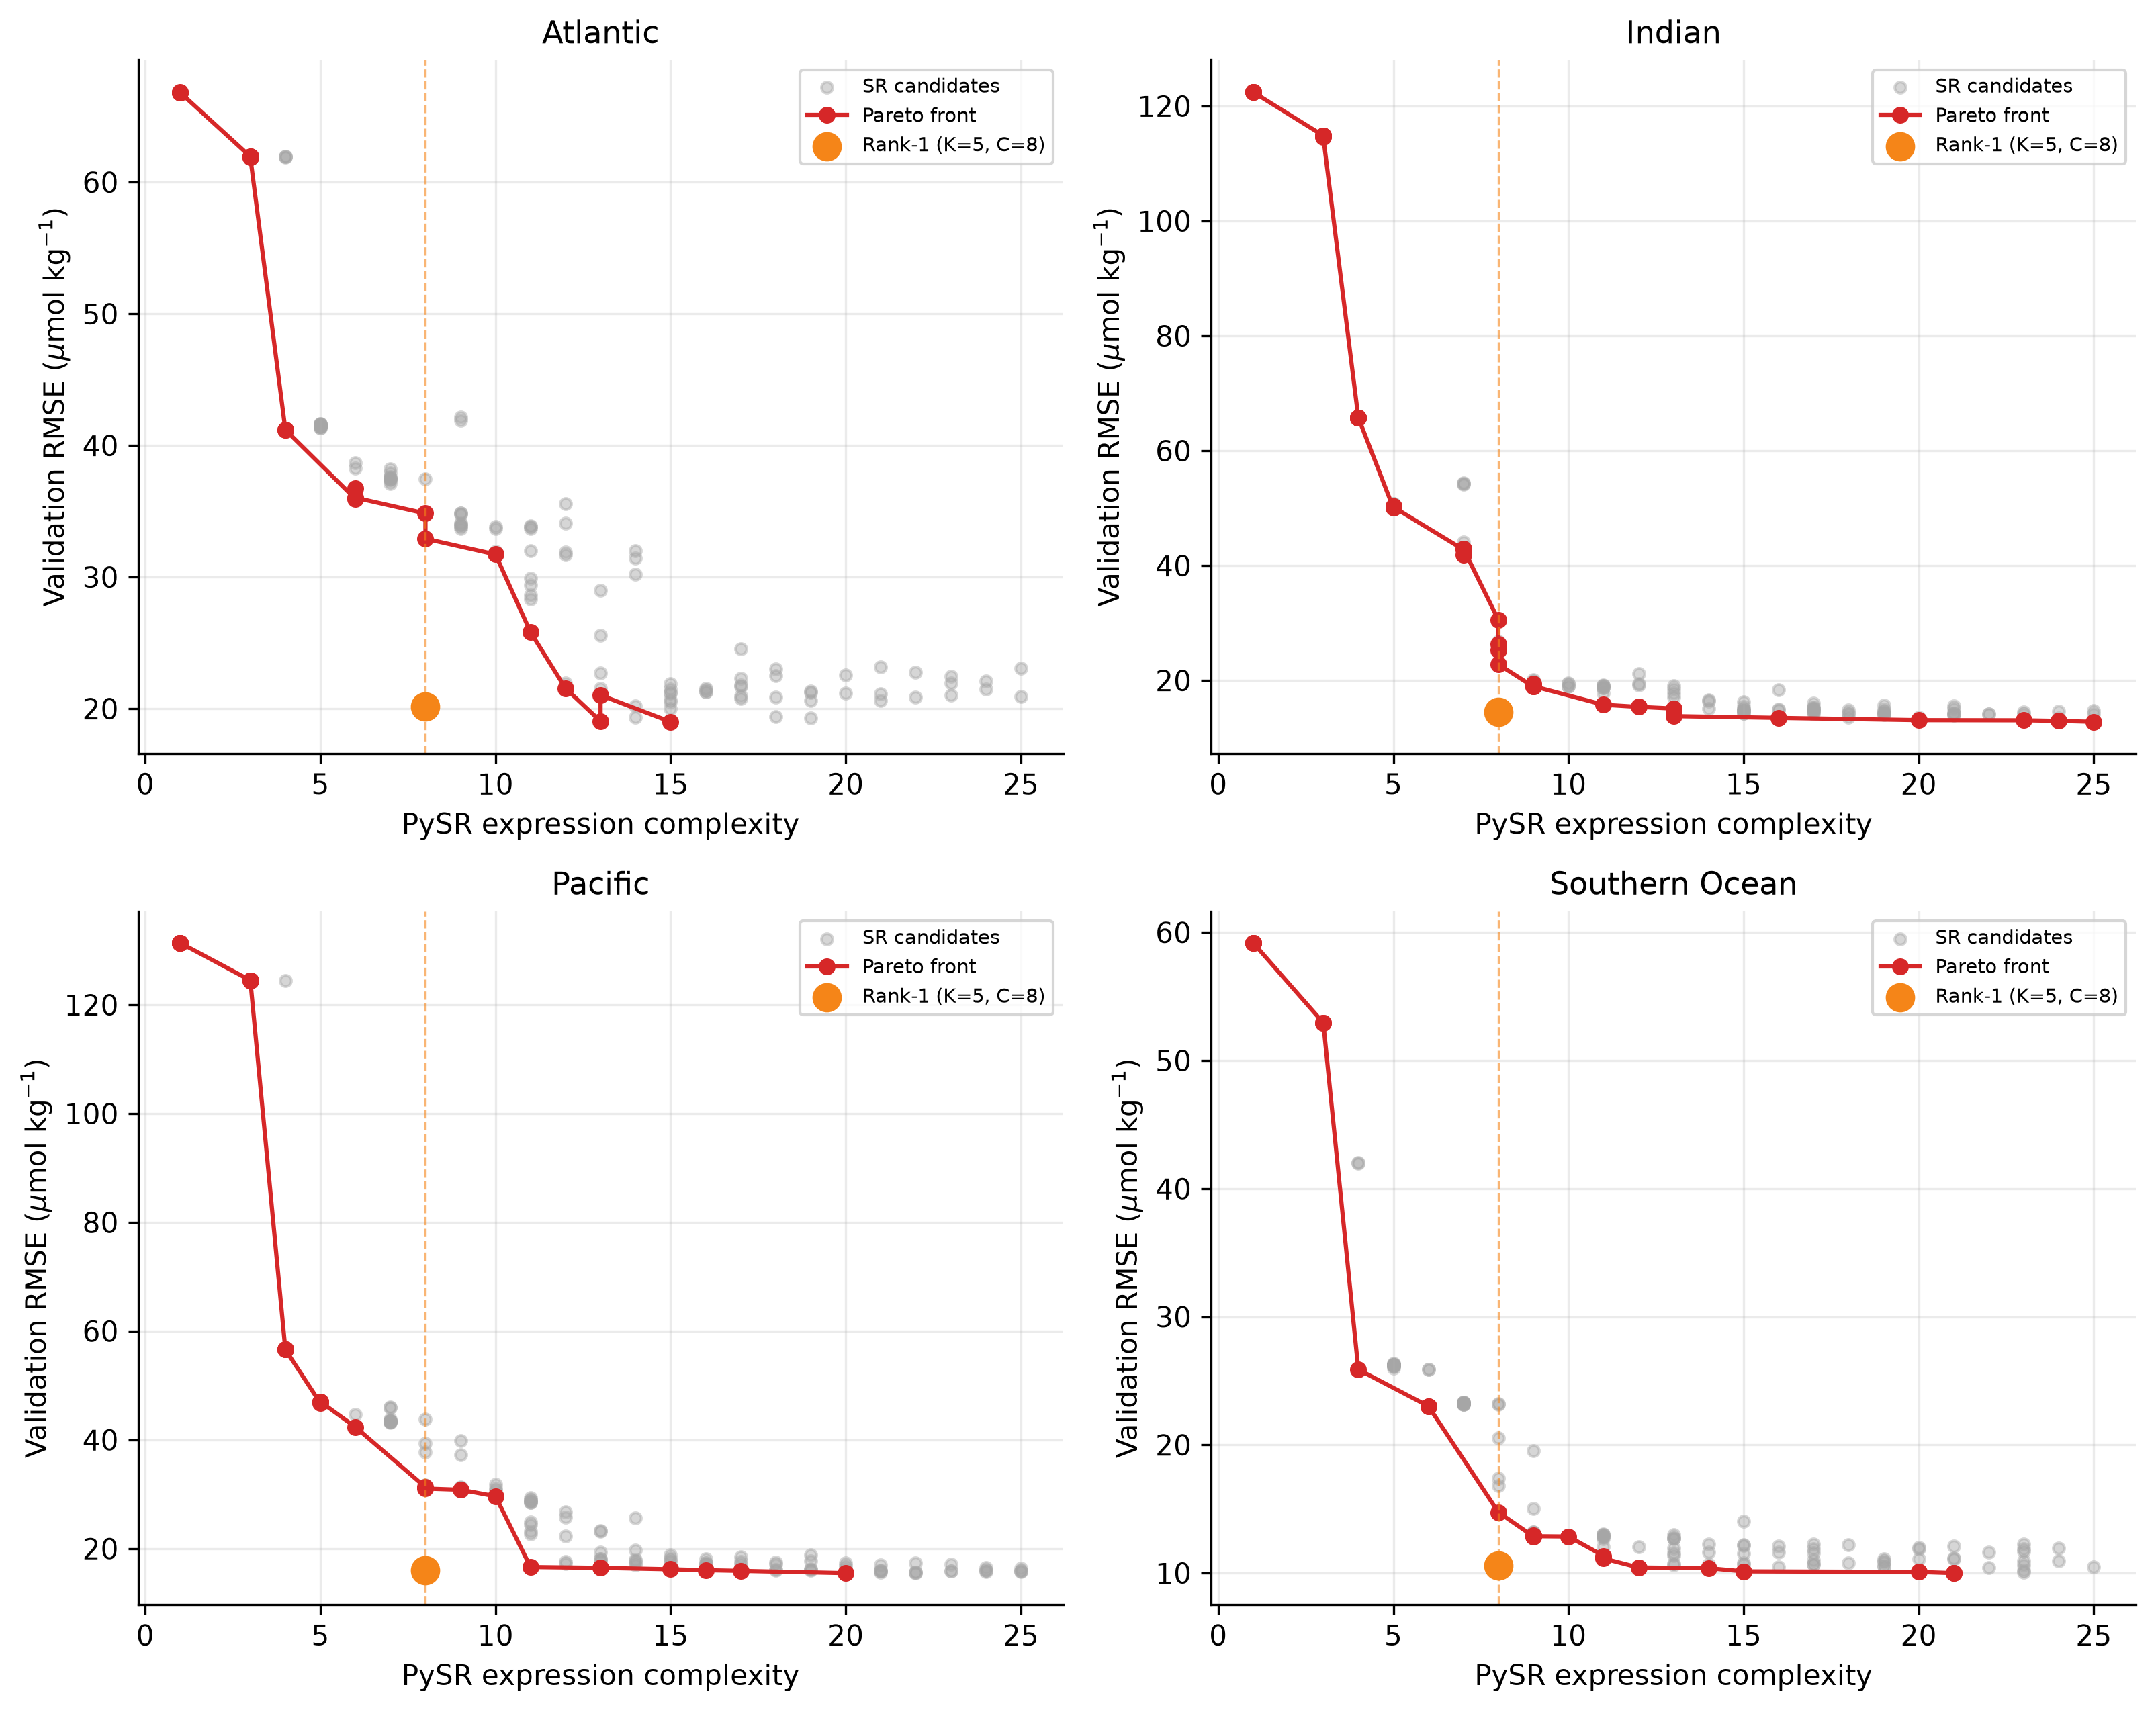
\includegraphics[width=0.9\textwidth]{figures/figure3_pareto_frontier.png}
\caption{Symbolic-regression validation RMSE versus PySR expression complexity. The vertical reference marks the rank-1 complexity ($C=8$). Higher-complexity candidates can reduce error, but expression complexity and fitted-parameter count are distinct quantities.}
\label{fig:pareto}
\end{figure}

\subsection{Temporal, spatial, cruise, and external generalization}
Table~\ref{tab:generalization} summarizes rank-1 performance across validation regimes. Spatial-block RMSE was 16.299, 16.609, 16.031, and 9.157~$\umol$ across the four basins; cruise-block RMSE was 16.910, 17.394, 16.031, and 9.225~$\umol$. Rankings changed across schemes: for example, in Atlantic spatial validation, rank-2 and full quadratic outperformed rank-1 even though rank-1 was better under the primary temporal split.

The locked post-2018 results support temporal transfer within the sampled distribution (Table~\ref{tab:generalization}). Neither blocked design establishes arbitrary geographic extrapolation.

\begin{table}[htbp]
\centering
\caption{Selected regional diagnostics. Water-mass values are from the Atlantic temporal-validation subset; abyssal values compare a global Southern Ocean fit with a local abyssal refit.}
\label{tab:regional}
\small
\begin{tabular}{llrrrr}
\toprule
Regime & Model & $N$ & RMSE & Bias & $R^2$ \\
\midrule
AAIW & Rank-1 & 428 & 28.426 & +27.143 & -0.115 \\
AAIW & Full quadratic & 428 & 22.333 & +21.126 & 0.312 \\
NADW & Rank-1 & 2,693 & 9.767 & -2.701 & 0.660 \\
Abyss, global & Rank-1 & 855 & 7.447 & +5.876 & -0.174 \\
Abyss, local refit & Rank-1 & 855 & 3.182 & --- & 0.786 \\
\bottomrule
\end{tabular}
\end{table}

\begin{table}[htbp]
\centering
\caption{Rank-1 RMSE across validation regimes. Spatial blocks are $5^{\circ}\times10^{\circ}$; cruise blocks use the available cruise identifier. Units are $\mu\mathrm{mol}\,\mathrm{kg}^{-1}$.}
\label{tab:generalization}
\small
\begin{tabular}{lrrrr}
\toprule
Basin & Temporal & Spatial block & Cruise block & External $\geq2018$ \\
\midrule
Atlantic & 20.172 & 16.299 & 16.910 & 17.672 \\
Indian & 14.483 & 16.609 & 17.394 & 18.413 \\
Pacific & 16.002 & 16.031 & 16.031 & 13.821 \\
Southern Ocean & 10.575 & 9.157 & 9.225 & 8.985 \\
\bottomrule
\end{tabular}
\end{table}

\begin{figure}[htbp]
\centering
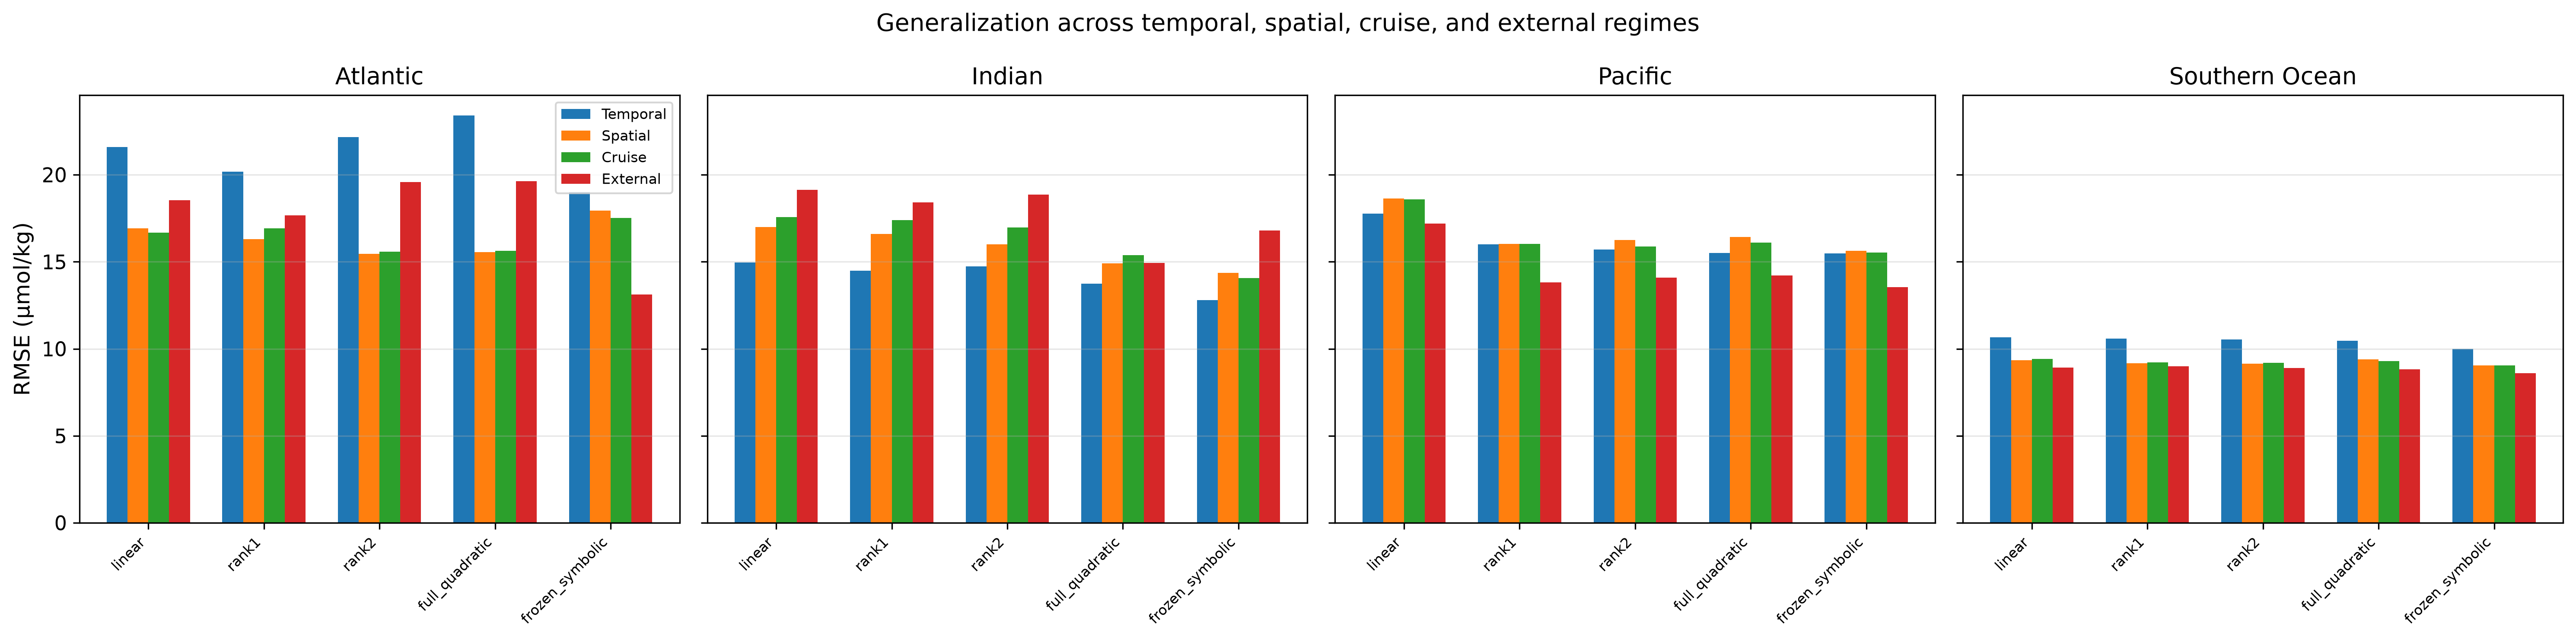
\includegraphics[width=\textwidth]{figures/figure4_generalization.png}
\caption{RMSE for linear, rank-1, rank-2, full-quadratic, and selected frozen symbolic models under temporal, spatial-block, cruise-block, and locked external evaluation. Rankings vary with validation regime.}
\label{fig:generalization}
\end{figure}

\subsection{Regional and water-mass limitations}
Errors were strongly regime-dependent. In the Atlantic threshold-based water-mass analysis, rank-1 RMSE was 28.426~$\umol$ with bias +27.143~$\umol$ for AAIW ($N=428$), whereas the full quadratic had RMSE 22.333~$\umol$ and bias +21.126~$\umol$. NADW was substantially better predicted by rank-1 (RMSE 9.767~$\umol$, bias $-2.701~\umol$, $N=2,693$). The contrasting AAIW and NADW results emphasize that basin-average performance does not describe all water-mass regimes.

The Southern Ocean abyss provides a sharper transferability test. For observations deeper than 3000 m and colder than $1\,^{\circ}\mathrm{C}$, the globally fitted rank-1 model had $R^2=-0.174$ and RMSE 7.447~$\umol$. A rank-1 model refit to the local abyssal training subset achieved $R^2=0.786$ and RMSE 3.182~$\umol$. The contrast is consistent with coefficient-transfer failure or domain shift; it does not show that abyssal $\tco$ is intrinsically unpredictable.

\begin{figure}[htbp]
\centering
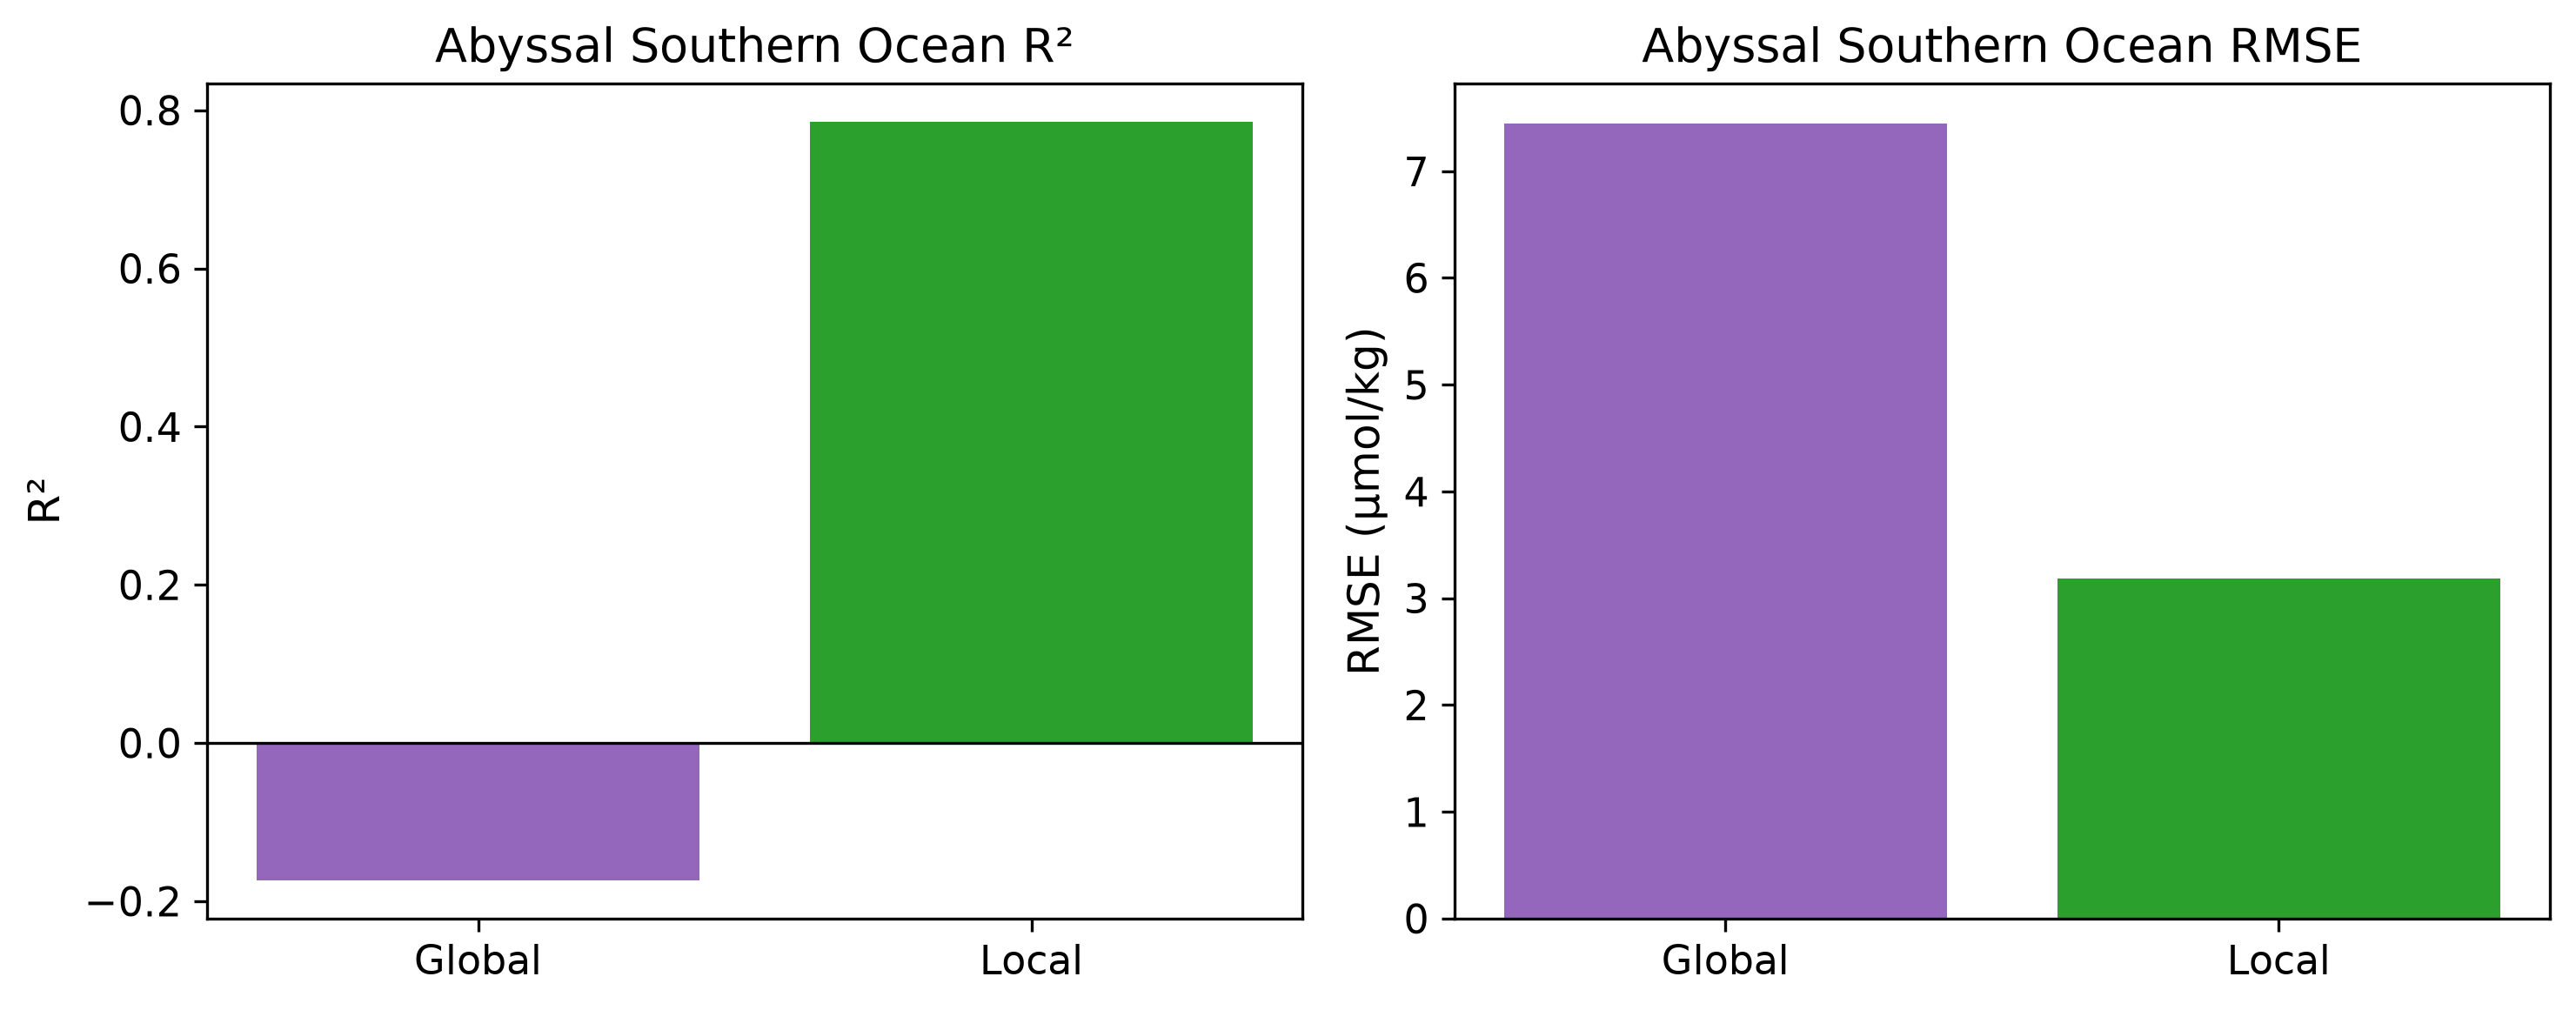
\includegraphics[width=0.8\textwidth]{figures/figure5_southern_abyss.png}
\caption{Southern Ocean abyssal performance for a basin-scale rank-1 fit and a local abyssal refit. The local improvement demonstrates domain dependence of the coefficients.}
\label{fig:abyss}
\end{figure}
